% /* cSpell:disable */
%  57205*2 - 11.7733    (ansys 2nd)

% mlp
% 262 - 11.7237
% 940 - 11.7598
% 1408 - 11.7670
% 2176 - 11.7704
% err=abs([11.7237,11.7598,11.7671,11.7704]-11.7733)/11.7733; dof=[262,940,1434,2176]; polyfit(log(dof),log(err),1)

% disperr > 0.005
% 262 - 11.7237
% 664 - 11.7513
% 1112 - 11.7649
% 1316 - 11.7670
% err=abs([11.7237,11.7513,11.7649,11.7670]-11.7733)/11.7733; dof=[262,664,1112,1316]; polyfit(log(dof),log(err),1)

% strerr > 0.01
% 262 - 11.7237
% 860 - 11.7552
% 2792 - 11.7691
% err=abs([11.7237,11.7552,11.7691,]-11.7733)/11.7733; dof=[262,860,2792]; polyfit(log(dof),log(err),1)

% ansys
% 69*2 -> 11.6574
% 241*2 ->  11.7397
% 897*2 -> 11.7646  
% 3457*2 -> 11.7711
% err_a1=abs([11.6574,11.7397,11.7646,11.7711]-11.7733)/11.7733; dof_a1=[69,241,897,3457]*2; polyfit(log(dof_a1),log(err_a1),1)
% /* cSpell:enable */
\subsection{Infinite plate with a circular hole}
\paragraph{}
In this example, an infinite plate with a traction free hole under uniaxial tension $(\sigma = \SI{1}{\newton \per \meter^2} ) $ along y-axis (see Fig.~\ref{adap_fig:ex_chole_geo_bc}) is considered.
\begin{figure}[h!]
    \centering
    \scalebox{1.4}{
        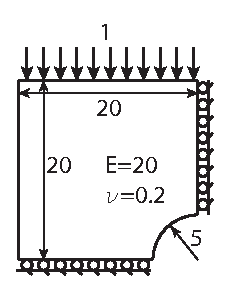
\includegraphics{adaptivity/ex_images/ex_chole_adap_geo_bc.eps}
    }
    \caption{Infinite plate with a circular hole: geometry and boundary conditions}
    \label{adap_fig:ex_chole_geo_bc}
\end{figure}

\paragraph{}
Owing to symmetry, only one quarter of the plate is modeled.
In this example, uniform distributed loads are applied on the top and plane stress condition is assumed.
The bottom and right boundaries are enforced with roller boundary conditions.
$u_y=0$ where $y=0$ and $u_x=0$ where $x=0$.

\paragraph{}
% result analysis
The rate of convergence in terms of the total strain energy is shown in Fig.~\ref{adap_fig:ex_chole_conv} and corresponding mesh development are presented in Fig.~\ref{adap_fig:ex_chole_mesh_sbfem} (SBFEM) and Fig.~\ref{adap_fig:ex_chole_mesh_ansys} ( Ansys 4-node quadrilateral element ).
Higher convergence rate compared to the result determined in ANSYS is observed.
\begin{figure}[h!]
    \centering
    \scalebox{0.6}{
        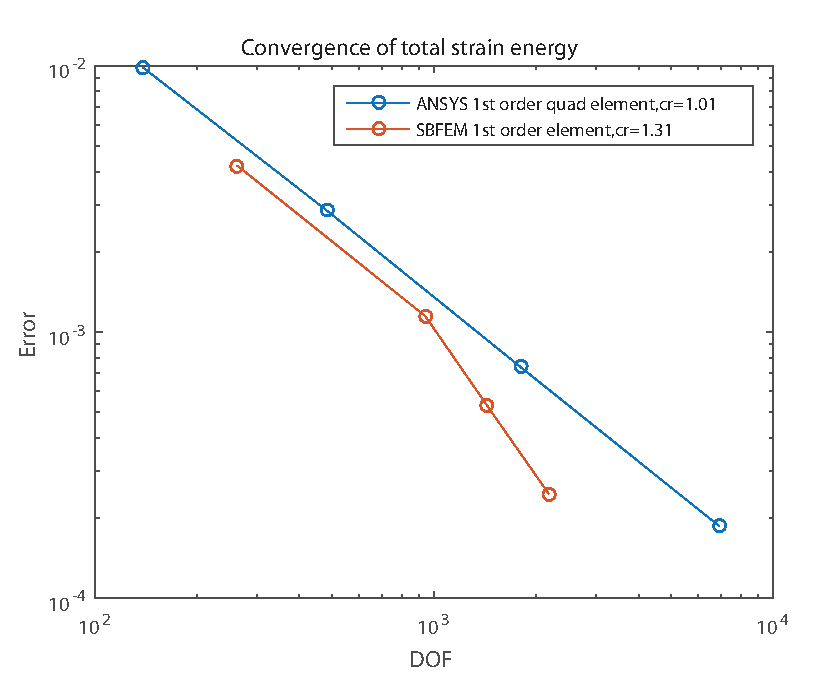
\includegraphics{adaptivity/ex_images/ex_chole_adap_conv.eps}
    }
    \caption{Infinite plate with a circular hole: Convergence study}
    \label{adap_fig:ex_chole_conv}
\end{figure}

\begin{figure}[h!]
    \centering
    \begin{subfigure}[b]{0.4\linewidth}
        \centering
        \scalebox{0.3}{
            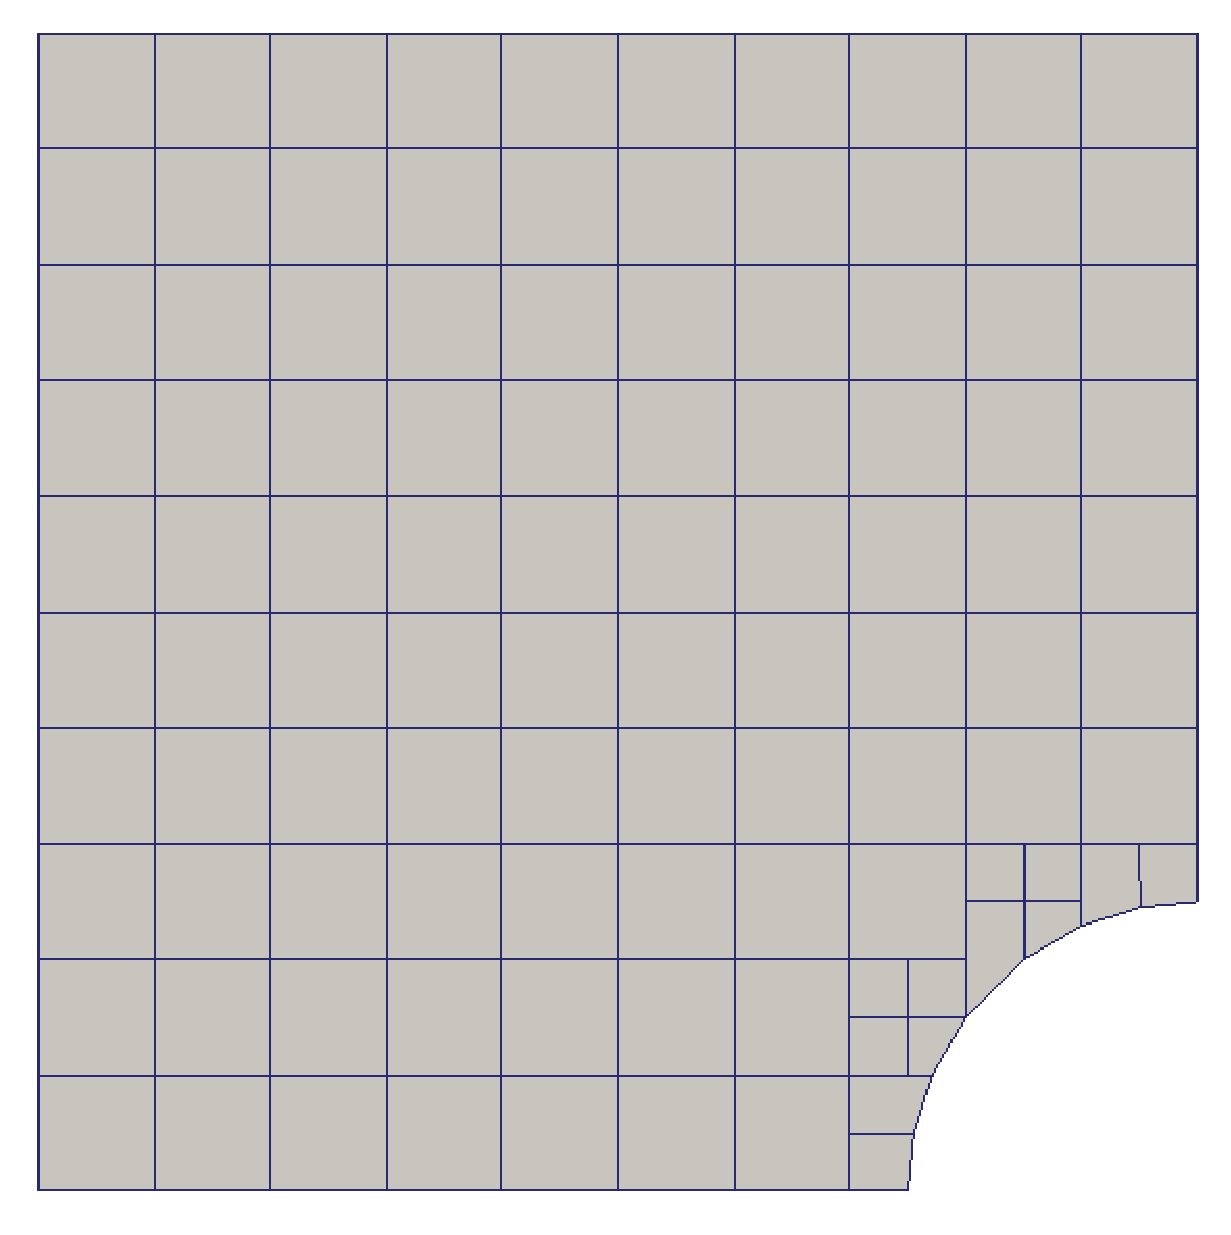
\includegraphics{adaptivity/ex_images/ex_chole_adap_131.eps}
        }
        \caption{Initial mesh, 131 DOFs}
    \end{subfigure}
    \begin{subfigure}[b]{0.4\linewidth}
        \centering
        \scalebox{0.3}{
            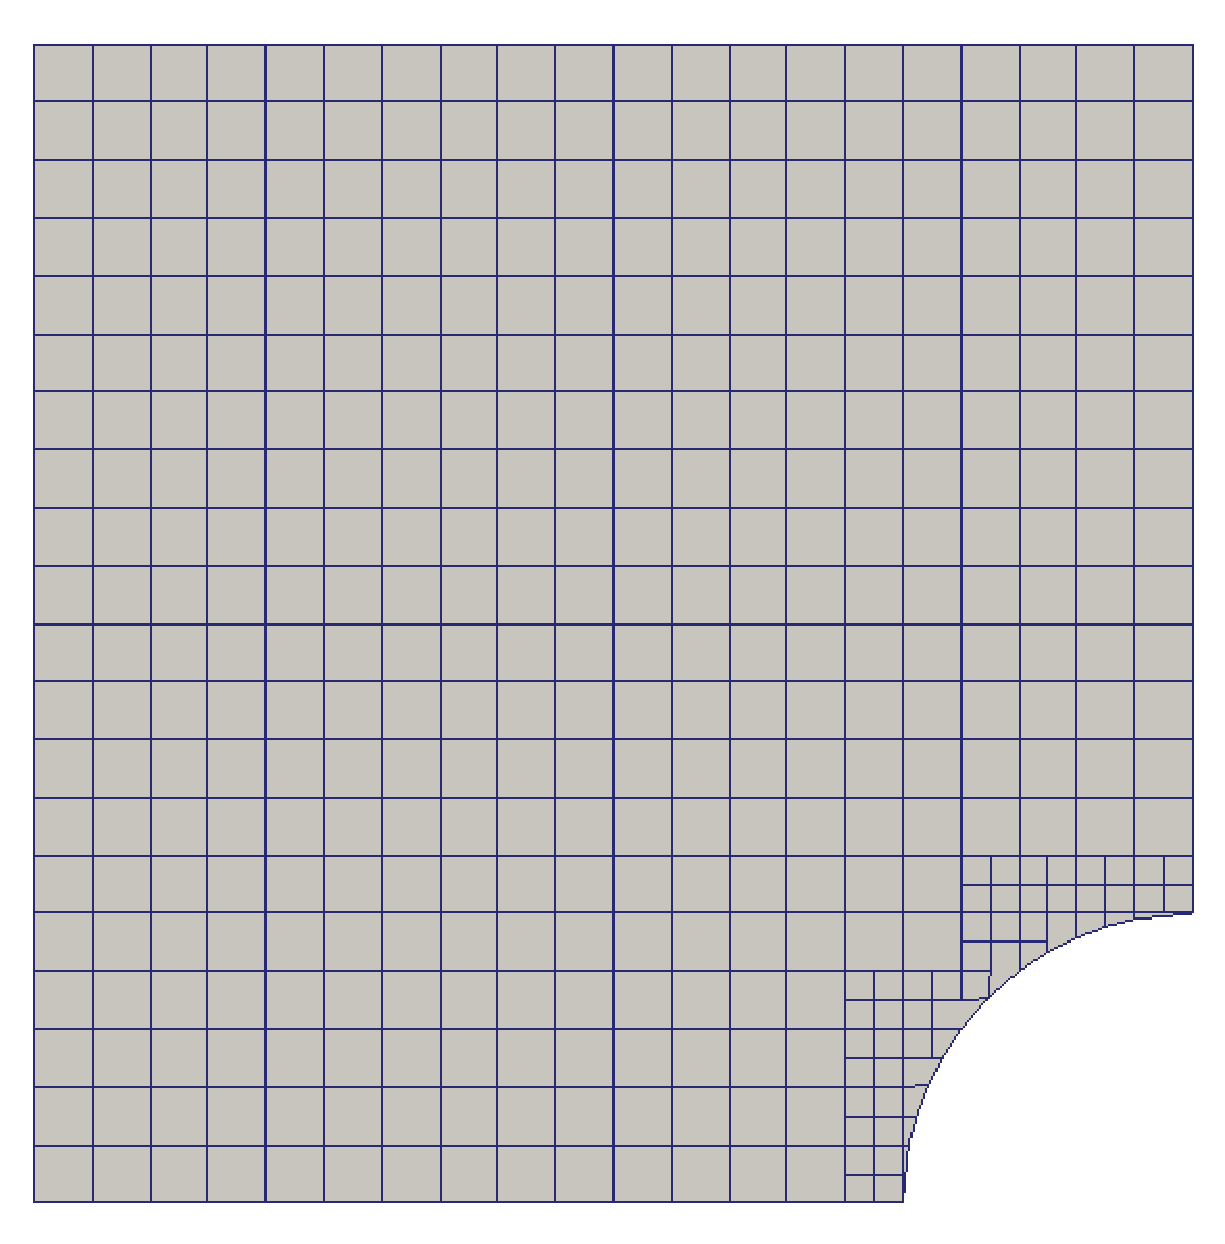
\includegraphics{adaptivity/ex_images/ex_chole_adap_472.eps}
        }
        \caption{1st refinement, 472 DOFs}
    \end{subfigure}
    \begin{subfigure}[b]{0.4\linewidth}
        \centering
        \scalebox{0.3}{
            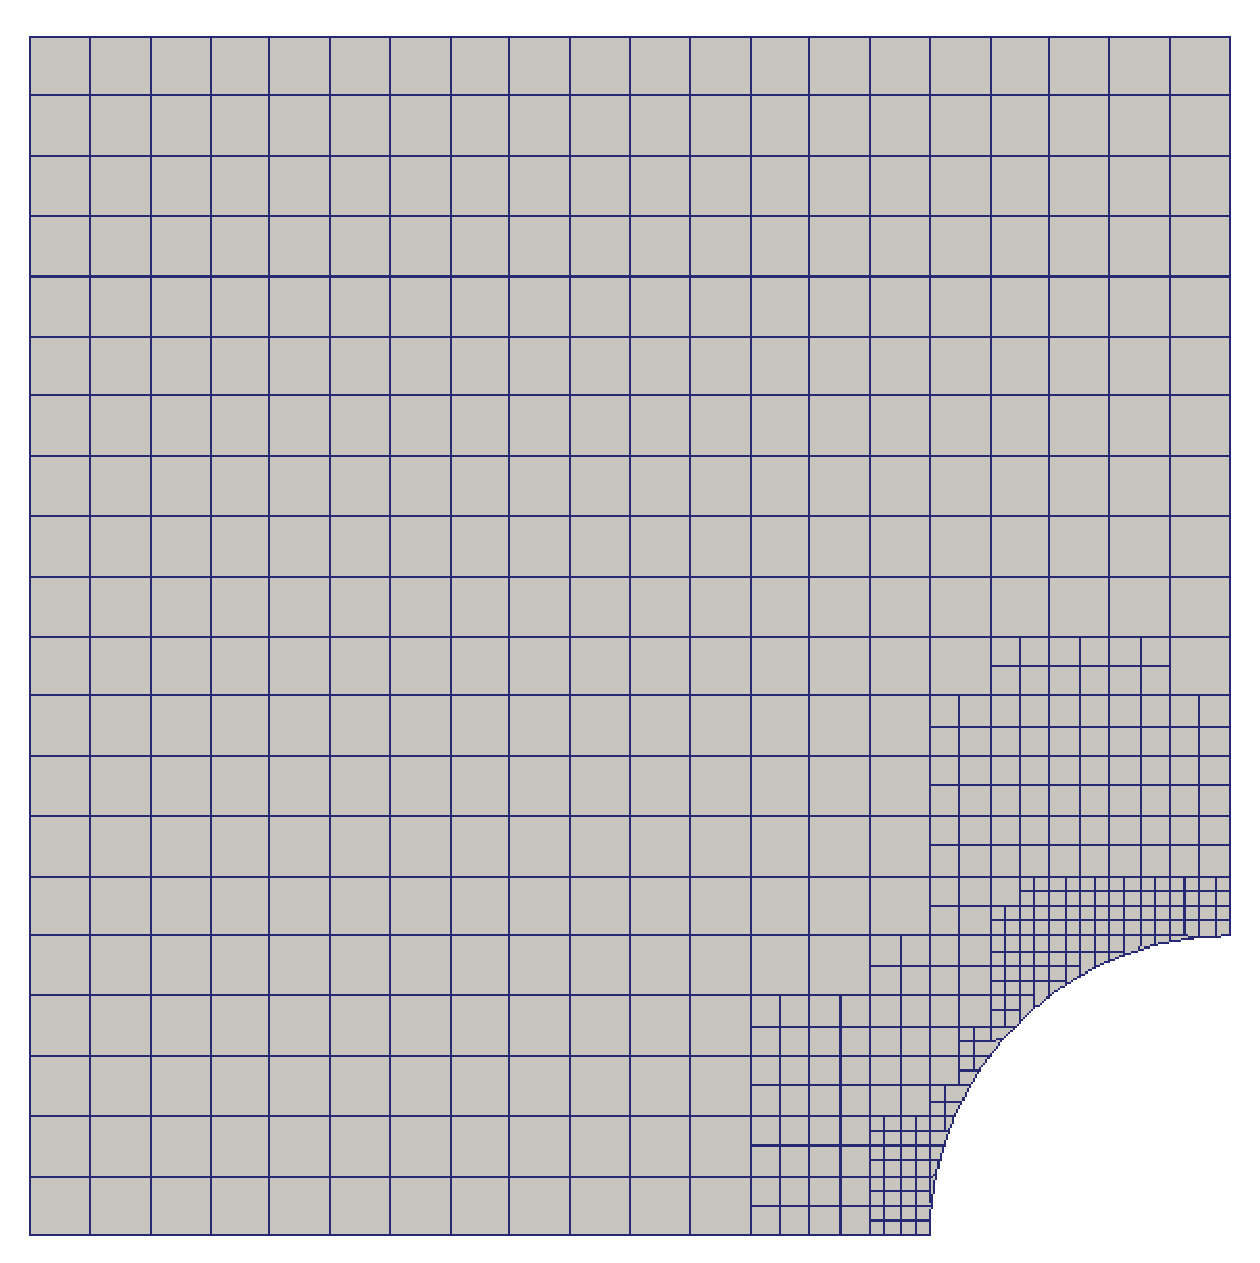
\includegraphics{adaptivity/ex_images/ex_chole_adap_700.eps}
        }
        \caption{2nd refinement, 700 DOFs}
    \end{subfigure}
    \begin{subfigure}[b]{0.4\linewidth}
        \centering
        \scalebox{0.3}{
            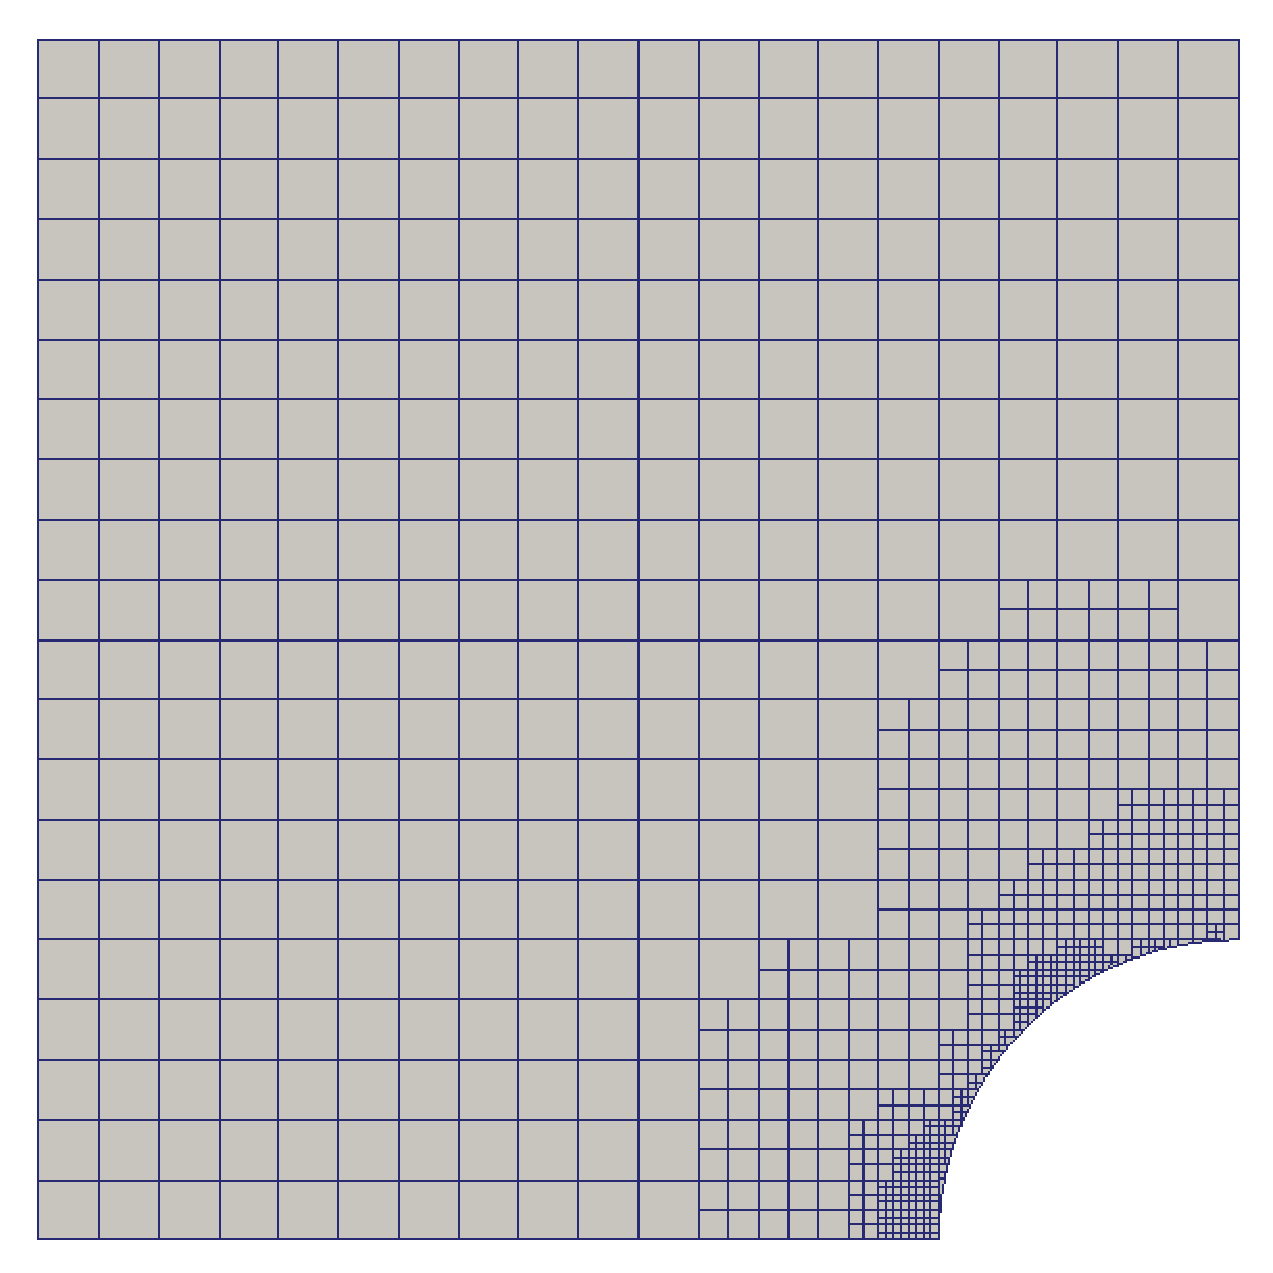
\includegraphics{adaptivity/ex_images/ex_chole_adap_1075.eps}
        }
        \caption{3rd refinement, 1075 DOFs}
    \end{subfigure}
    \caption{Infinite plate with a circular hole: Mesh development (SBFEM)}
    \label{adap_fig:ex_chole_mesh_sbfem}
\end{figure}

\begin{figure}[h!]
    \centering
    \begin{subfigure}[b]{0.48\linewidth}
        \centering
        \scalebox{0.4}{
            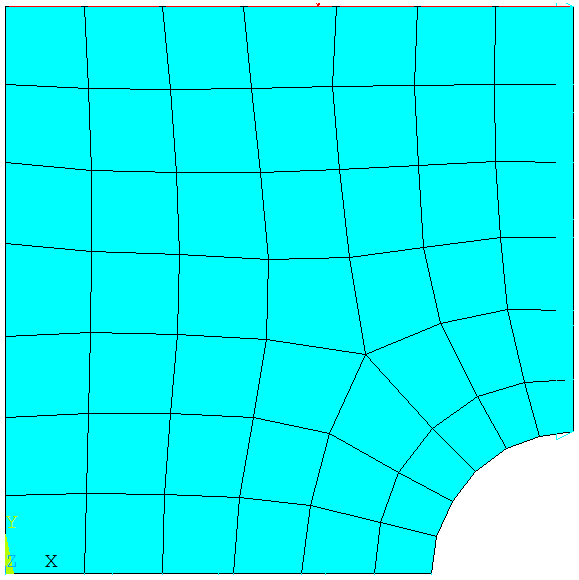
\includegraphics{adaptivity/ex_images/ex_chole_ansys_1_69.png}
        }
        \caption{Initial mesh, 138 DOFs}
    \end{subfigure}
    \begin{subfigure}[b]{0.48\linewidth}
        \centering
        \scalebox{0.4}{
            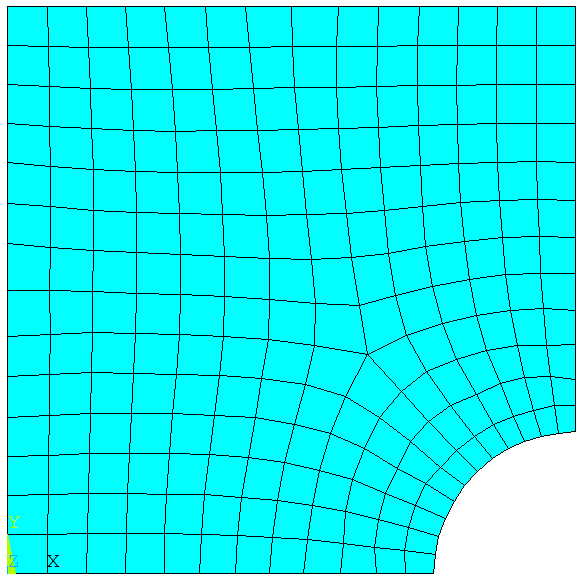
\includegraphics{adaptivity/ex_images/ex_chole_ansys_1_241.png}
        }
        \caption{1st refinement, 482 DOFs}
    \end{subfigure}
    \begin{subfigure}[b]{0.48\linewidth}
        \centering
        \scalebox{0.4}{
            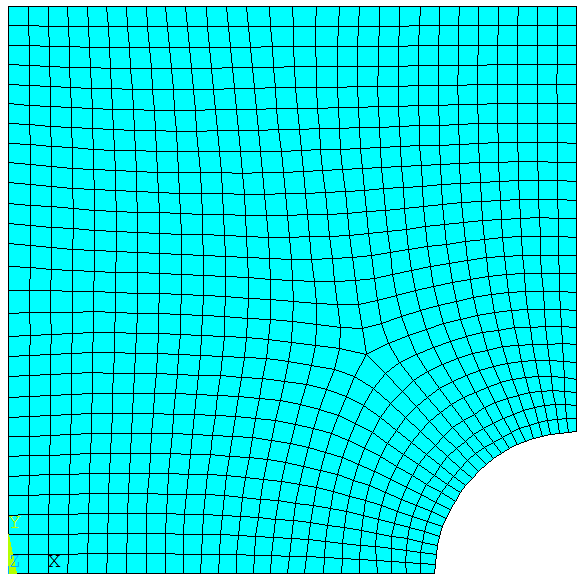
\includegraphics{adaptivity/ex_images/ex_chole_ansys_1_897.png}
        }
        \caption{2nd refinement, 1794 DOFs}
    \end{subfigure}
    \begin{subfigure}[b]{0.48\linewidth}
        \centering
        \scalebox{0.4}{
            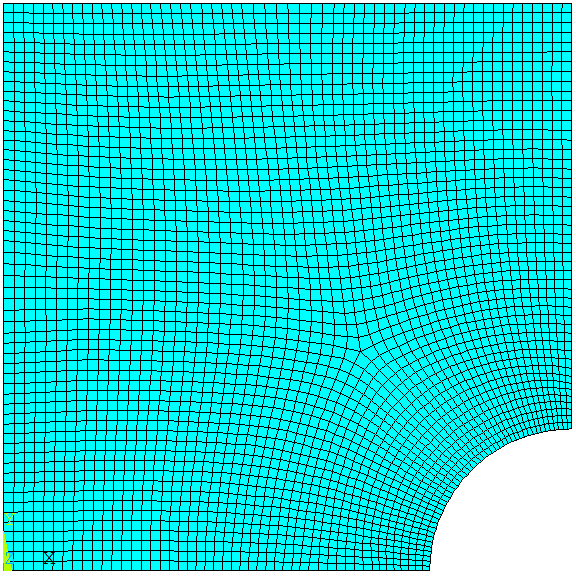
\includegraphics{adaptivity/ex_images/ex_chole_ansys_1_3457.png}
        }
        \caption{3rd refinement, 6914 DOFs}
    \end{subfigure}
    \caption{Infinite plate with a circular hole: Mesh development (Ansys)}
    \label{adap_fig:ex_chole_mesh_ansys}
\end{figure}

\begin{figure}
    \centering
    \scalebox{0.5}{
        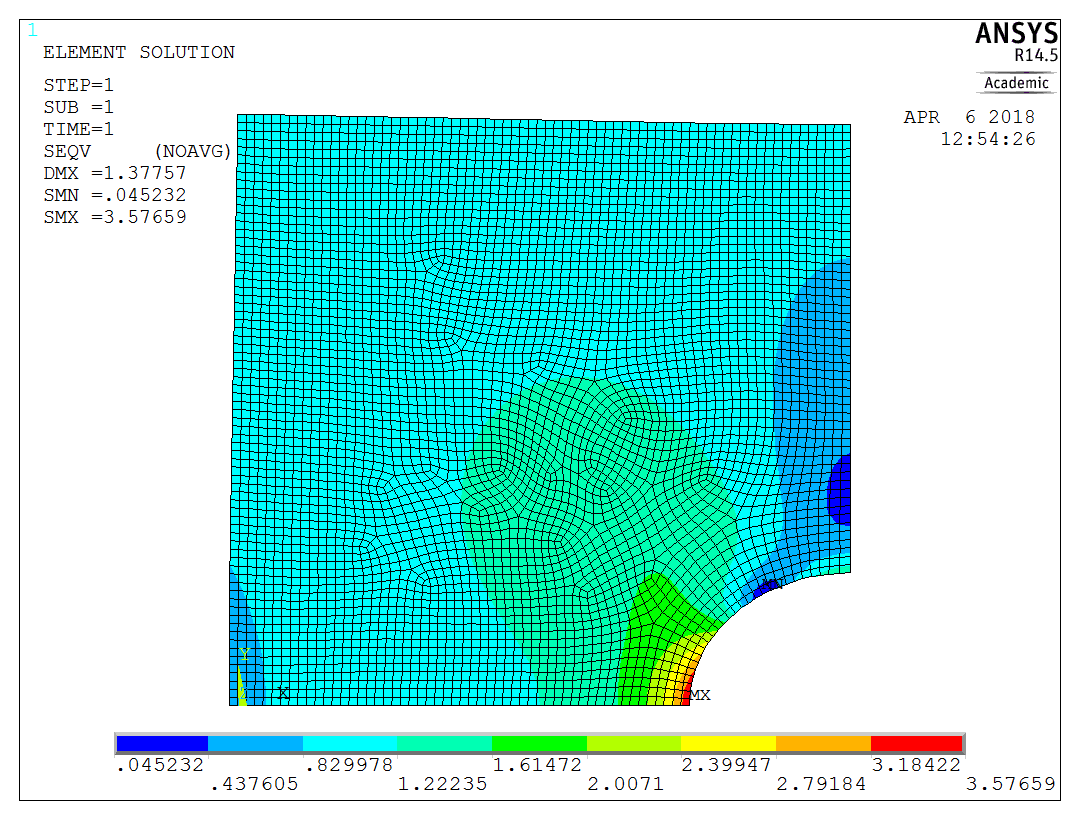
\includegraphics{adaptivity/ex_images/ex_chole_stress_ansys.png}
    }
    \caption[Von-mises stress contour using 9-node quadrilateral element in ANSYS]{Von-mises stress contour using 9-node quadrilateral element in ANSYS (28450 DOFs)}
    \label{adap_fig:ex_chole_stress_ansys}
\end{figure}
